\chapter{Data Reduction and Analysis}
	\label{cha:Data}
This chapter presents the observations of the Southern Sample (as laid out in Section \ref{sec:Sample}) made with the VIsable Multi-Object Spectrograph (VIMOS; see Section \ref{sec:VIMOS}). The data-reduction pipeline is laid out in Section \ref{subsec:VIMOSreduction} with a discussion of the data quality, including the artifacts from the VIMOS instrument, in Section \ref{subsec:VIMOSartifacts}. A brief discussion of alternative data-reduction pipeline for VIMOS is given in Section \ref{subsec:Other}. Unpublished, archival observations made with the Multi-Unit Spectroscopic Explorer (MUSE) that are also used in this project are described in Section \ref{sec:MUSE}. This includes a discussion of the European Southern Observatory's (ESO's) data-reduction pipeline (Section \ref{subsec:MUSEreduction}). Finally, in Section \ref{sec:analysis}, we describe the data-analysis pipelines, which are used to produce the results presented in Chapters \ref{cha:stellar} and \ref{cha:gas}.  

\section{The VIsable Multi-Object Spectrograph (VIMOS)}
	\label{sec:VIMOS}
	\subsection{The VIMOS Instrument}
		VIMOS is a fibre-fed, multi-purpose spectrograph mounted on Unit Telescope 3 (UT3) on the European Southern Observatory's (ESO's) Very Large Telescope (VLT) in Paranal, Chile \citep{LeFevre2003}. It operates in a number of configurations: direct imaging, multi-object spectroscopy (MOS) or integral-field spectroscopy (IFS). For this program, VIMOS was used in IFS mode. 

		The integral-field unit (IFU) has a field of view of 40 x 40 spatial pixels (spaxels) with a choice of sampling of 0.67" or 0.33". There are 6 available grisms with varying wavelength ranges and spectral resolutions: low- or high-resolution (LR or HR) red; HR orange; and LR, medium resolution (MR) or HR blue. The observations presented in the following Section were taken using the new (at the time) HR blue grism with a spatial resolution of 0.67". 

		The field of view of VIMOS is split into 4 quadrants (named in the fits headers, perhaps unhelpfully: Brian, Keith, Tom and David). The quadrants are run in parallel as independent detectors (it is not possible to use different grisms with different quadrants). Fibres are arranged in a row along the short side of the charge-coupling device (CCD) detectors, and the light from each fibre is dispersed by the grism in the other direction. This gives rise the row-stack spectra (RSS) format of most IFU devices.

		VIMOS has several well known, though poorly understood technical issues. These include several low transmission (bad) fibers, strong flexure and large differences in sensitivity across its 4 separate detectors, known as quadrants. These are addressed by a specialist data reduction pipeline as described in Section \ref{subsec:VIMOSreduction} with a discussion of the resulting data quality in Section \ref{subsec:VIMOSartifacts} (for more detail also see the instrument manual, section 2.8 in current version\footnote{http://www.eso.org/sci/facilities/paranal/instruments/vimos/doc.html}).

	\subsection{Observations With VIMOS}
		As stated above, the observations for this project were taken using the IFS mode (with at a spatial resolution of 0.67"), with the blue HR grism. This grism gives a wavelength range of 3700-5520\,\AA\ at a spectral resolution of 0.71\,\AA\,$\mathrm{pix^{-1}}$. 

		The program of observations (ID: 089.B-0632A) ran in service mode during ESO period 89 and 90. Each object was imaged with a total integration time of $\approx 100$ mins equally spread over three observing blocks (OBs). Each block contained all of the necessary calibration images (3 continuum lamp (flat field) exposures and 1 He and Ne arc lamp exposure for wavelength calibration), as well as two science pointings. In addition, VIMOS provides 5 bias images per night. Flux calibrations calculated using publicly available observations of Feige 110 provided by ESO. A summary of the observations are given in Table \ref{tab:observations}.

		


	\subsection{Data Reduction of VIMOS Data}
		\label{subsec:VIMOSreduction}
		The data reduction pipeline was produced using \textsc{Py3D}, a suite of programs based on the \textsc{python} versions of those developed for Califa \citep{Sanchez2012, Husemann2013} and later updated for VIMOS by \citet{Husemann2014}. \textsc{Py3D} was provided to us by Husemann (personal correspondence) and is (currently) not publicly available. It  makes use of pixel tables in order to track each pixel through the pipeline, with both spectral and spatial resampling only occurring once. This pipeline accounts for many of the known issues with VIMOS such as bad fibers, strong flexure and cross-talk as well as standard reduction procedures for IFS data. A full outline of the reduction is given here.

		A median master bias is created from the five daily bias frames and subtracted from each raw frame. Known low-transmission (bad) fibres, detected cosmic ray hits and offsets to account for flexure of the instrument due to gravity are taken into account when automatically identifying the fibre positions on the detector. The fibre is then traced along the dispersion axis in the flats. \citet{Husemann2014} finds this to be robust except for a few fibres at the very blue end of the spectrum ($<4300$\,\AA). 

		Since flexure is dependent on position angle of the telescope and rotation of the instrument, the exposures on the source (science exposures) will be affected in a different manner to the flat field exposures. \textsc{Py3D} accounts for the offset of the science exposure to the flat field exposure by tracing the peak fibre position directly on the science exposure at 5 or 6 locations. The offsets are then extrapolated with a second order Legendre polynomial. This corrects for the flexure in the fibre number direction, but flexure also affects the dispersion direction. The effect is estimated by the positions of strong emission lines from the atmosphere (sky lines), however the HR blue only has one sky line at 5199\,\AA, which in many of our science frames was very dim or even not present. This lack of sky lines had previously been an issue with our initial attempt at data reduction using the publicly available \textsc{p3d}\footnote{http://p3d.sourceforge.net/} program. Here the lack of sky lines meant \textsc{p3d} was not able to flux calibrate the quadrants to each other. For this reason (and the lack of accounting for the flexure of VIMOS), we converted to \textsc{Py3D}.

		Another issue taken into account by \textsc{Py3D} is cross-talk, where fibres are so densely packed that light from one fibre bleeds into the image of neighboring fibres. The spectra are extracted assuming a Gaussian profile for the cross-dispersion of each fibre with the width fitted for each fibre individually. After this, the spectra are adaptively smoothed to a 3\,\AA\ full-width, half-maximum (FWHM) resolution and resampled.

		Flats are used to correct for the different efficiencies of transmission of each fibre and sensitivities of each CCD pixel (flat-fielding). Observations of the standard star Feige 110, imaged in each of the 4 quadrants, are made automatically by ESO and are reduced in the same way as described above. Comparisons of the resulting spectra to a reference spectrum for Feige 110 (provided by Husemann; private correspondence) are used to flux calibrate each quadrant. A mean sky spectrum, built using spectra from the outer regions of the field of view of each quadrant, is then subtracted from the science frames. 

		The quadrant are combined into a single file, which was converted from the RSS format to a cube (with dimensions of RA, Dec. and wavelength, $\lambda$). Finally, the change in position of the centre of the galaxy due to differential atmospheric refection (DAR) is measured and corrected for. 

		\begin{figure}
			\centering
			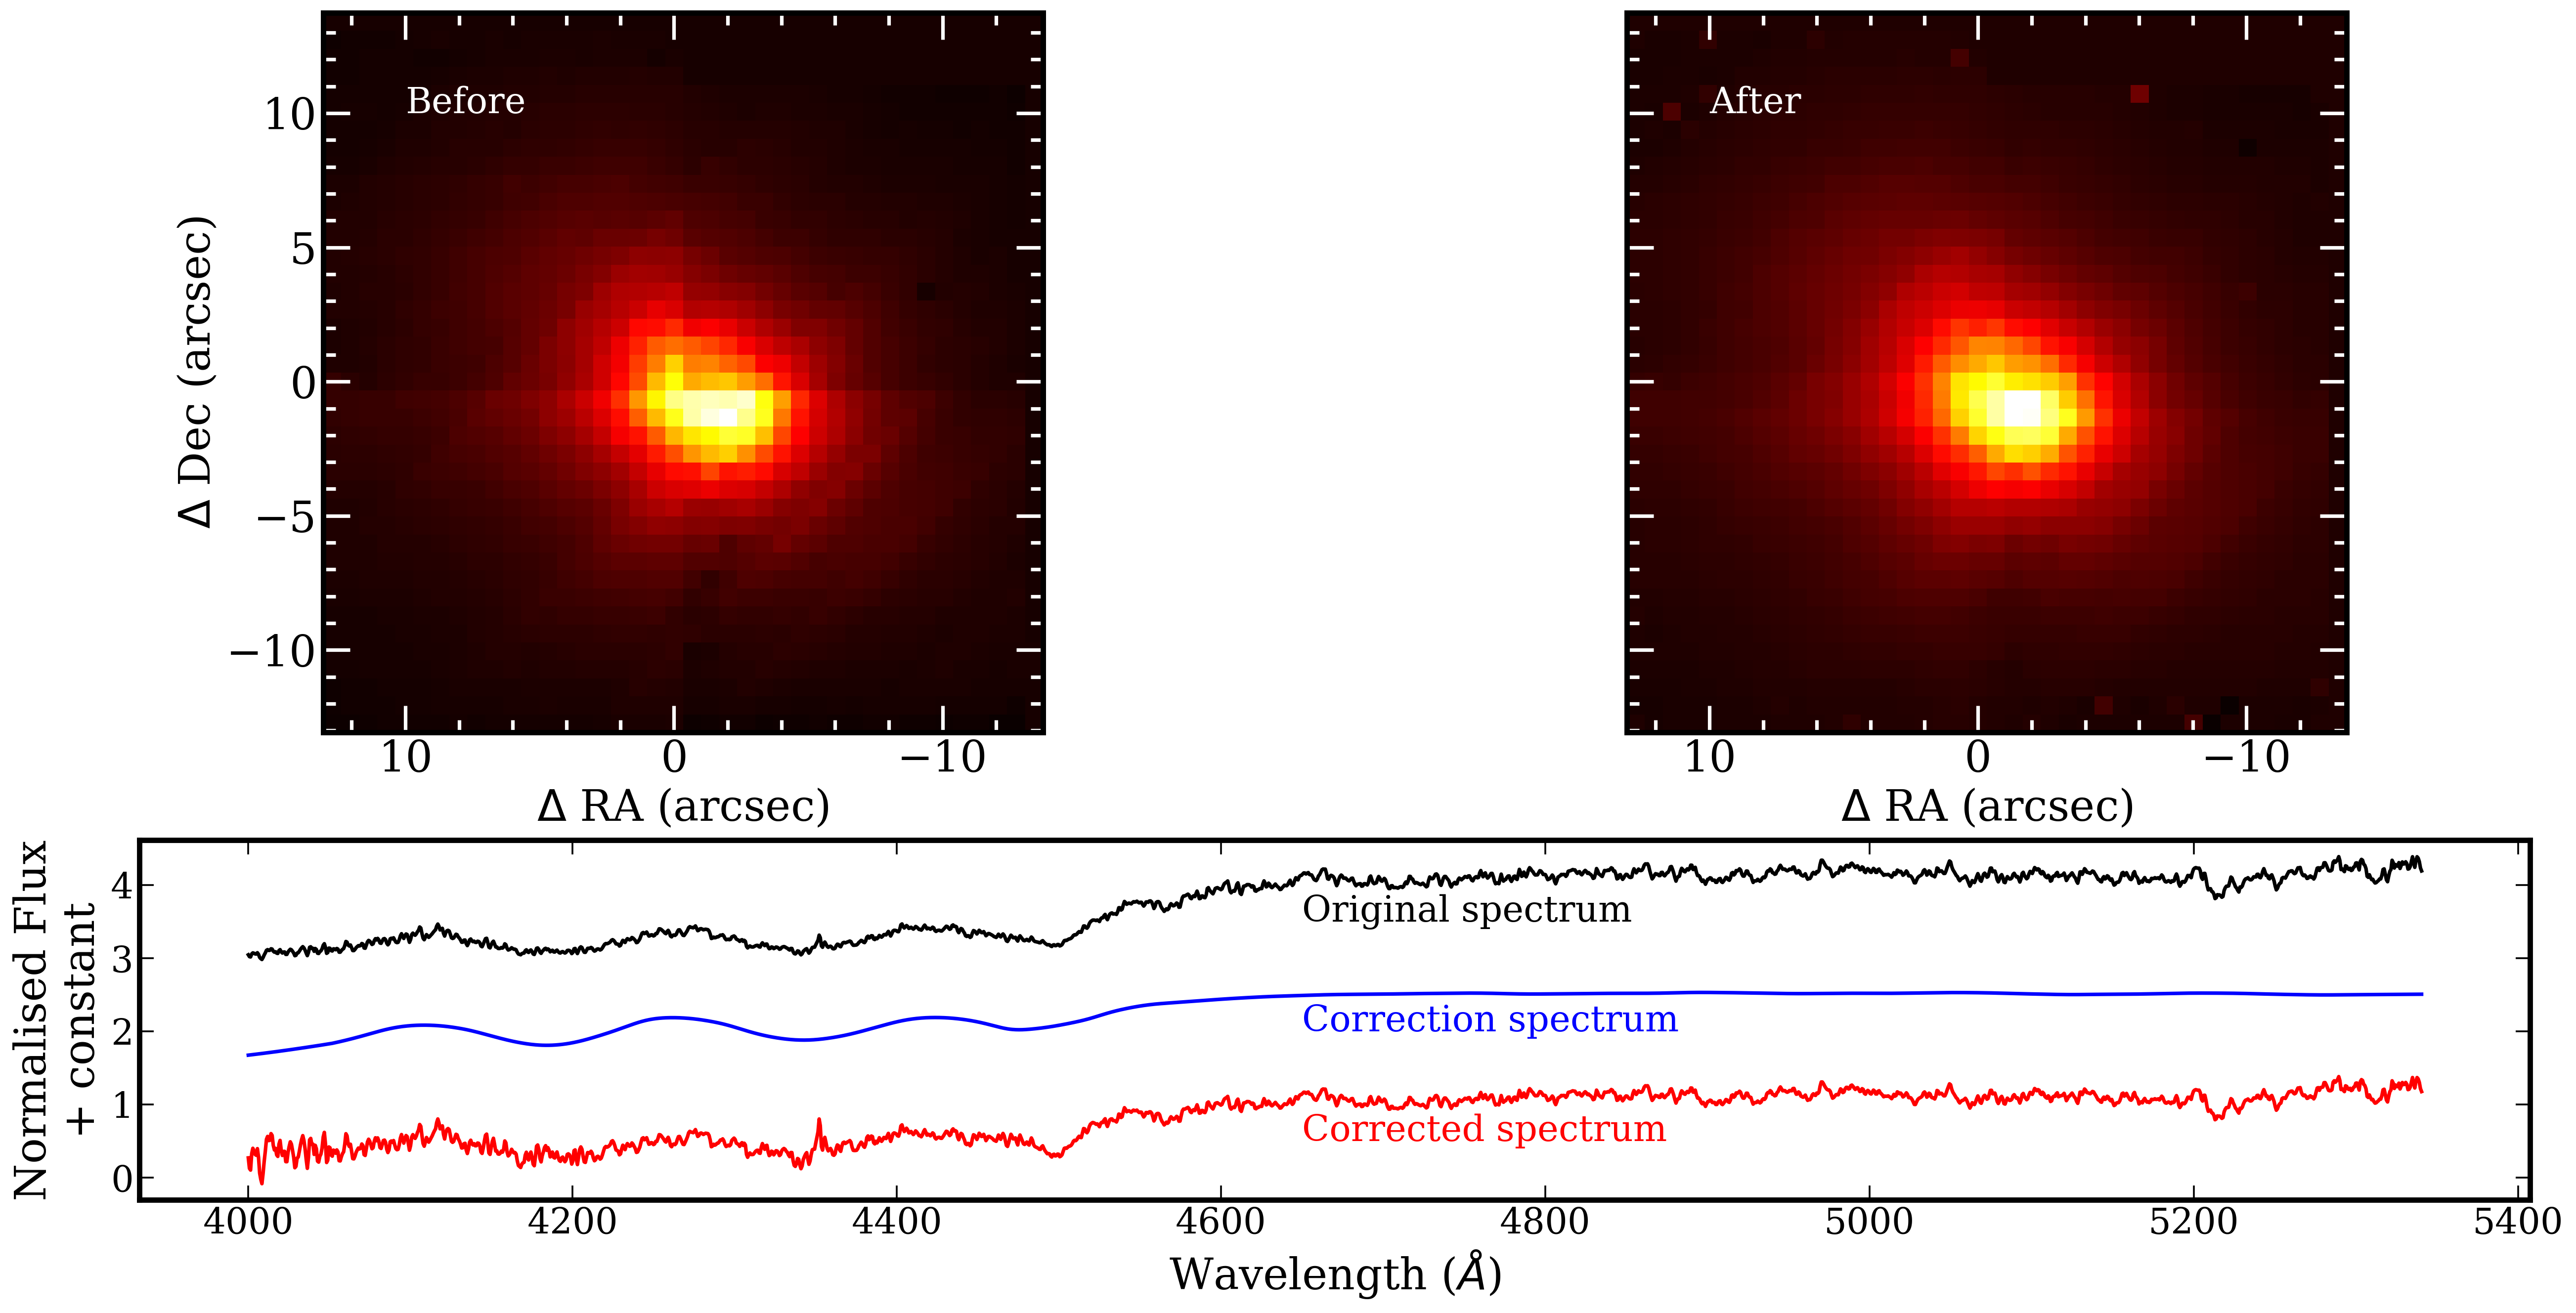
\includegraphics[width=0.99\textwidth]{chapter2/corr_image.png}
			\caption[Ad-hoc correction to VIMOS datacubes]{The affect of the ad-hoc corrections applied as part of the VIMOS data reduction pipeline. Top panels show before and after ad-hoc correction is applied to NGC 3557. The correction is aimed to improve the quadrant-to-quadrant calibration and reduce diagonal intensity strips. Bottom panel: an example of the correction applied to a single spaxel in NGC 3100 to correct for the fringe-like pattern.}
			\label{fig:Correction}
		\end{figure}

		Following on from this, we noted that the cubes where still not fully corrected. Three main issues remain: quadrants have different intensities, clearly showing an uncorrected difference in throughput; diagonal intensity stripes; and a fringe-like pattern was still observable in the spectral direction. The first two of these issues can be seen in the top left panel of Fig.\,\ref{fig:Correction}. \citet{Lagerholm2012} points out that the intensity strips do not seem to be bound to the quadrants. They conclude that the stripes therefore originate from an unknown reduction pipeline problem. They make use of the reduction pipeline supplied by ESO\footnote{http://www.eso.org/sci/software/pipelines/vimos/}, while we have used the independent \textsc{Py3D} and also observe the intensity stripes. This suggests that the pipeline may not be the cause. The fringe-like patterns appear to be due to position-angle and hysteresis dependent reflections occurring within the fibres. 

		These issues were corrected by implementing a \textsc{python} version of the ad-hoc corrections given in \citet{Lagerholm2012}. This involves re-normalizing the quadrants to each other by minimizing the difference of the integrated spectra in neighboring fibers along the edge of each quadrant (quadrant 2 was held constant). This is followed by the removal of the fringe-like pattern by dividing out a smoothed median spectrum from the eight surrounding fibers of any given fiber, over a scale of 150 pixels (example shown for a single spaxel in NGC 3100 in the bottom panel of Fig.\,\ref{fig:Correction}). The top two panels in Fig.\,\ref{fig:Correction} show the images (where the datacube is collapsed in the spectral direction) of NGC 3557 before and after these corrections are applied. These steps mean that the data-cubes are not perfectly flux-calibrated, however the effect is multiplicative and thus will not effect equivalent width measurements. From comparison the the MUSE data (Section \ref{sec:MUSE}) we estimate flux of the resulting datacubes to be in units of $\sim 10^{-15} \, \mathrm{erg\,s^{-1}\,cm^{-2}}$. 

		

		The variance spectra is propagated throughout the data reduction pipeline and square-rooted at this point, to be used a noise input in the analysis (Section \ref{sec:analysis})

	\subsection{Data Quality}
		\label{subsec:VIMOSartifacts}
		By comparing the top panels in Fig.\,\ref{fig:Correction}, we can clearly see that while there is an obvious improvement to the calibration between the quadrants, there is still a sharp transition. This often gives rise to characteristic diamond shaped isophotes, rather than ellipses. The neighboring spaxels along the transitions can have fluxes that are different by as much as 20-30\%. Luckily, the worst affected galaxies are IC 4296 and NGC 1399, for which we have MUSE archival data for (see Section \ref{sec:MUSE}). 

		Similar transitions are also observed in the spectral direction, with a slight offset in wavelength calibration between quadrants. This is most clearly seen in the mean velocity maps after the routines described in Section \ref{subsec:StellarFit} are applied. The left panel in Fig.\,\ref{fig:egVel} shows the mean velocity map for NGC 1399 and clearly shows the top-right quadrant to have a slightly higher velocity than would be expected for a normal rotating galaxy. This corresponds to a shift in the spectra. For comparison, the right panel of Fig.\,\ref{egVel} shows the mean velocity map from a different instrument which does not suffer from this issue. Again the worst affected galaxies are IC 4296 and NGC 1399.

		\begin{figure}
			\centering
			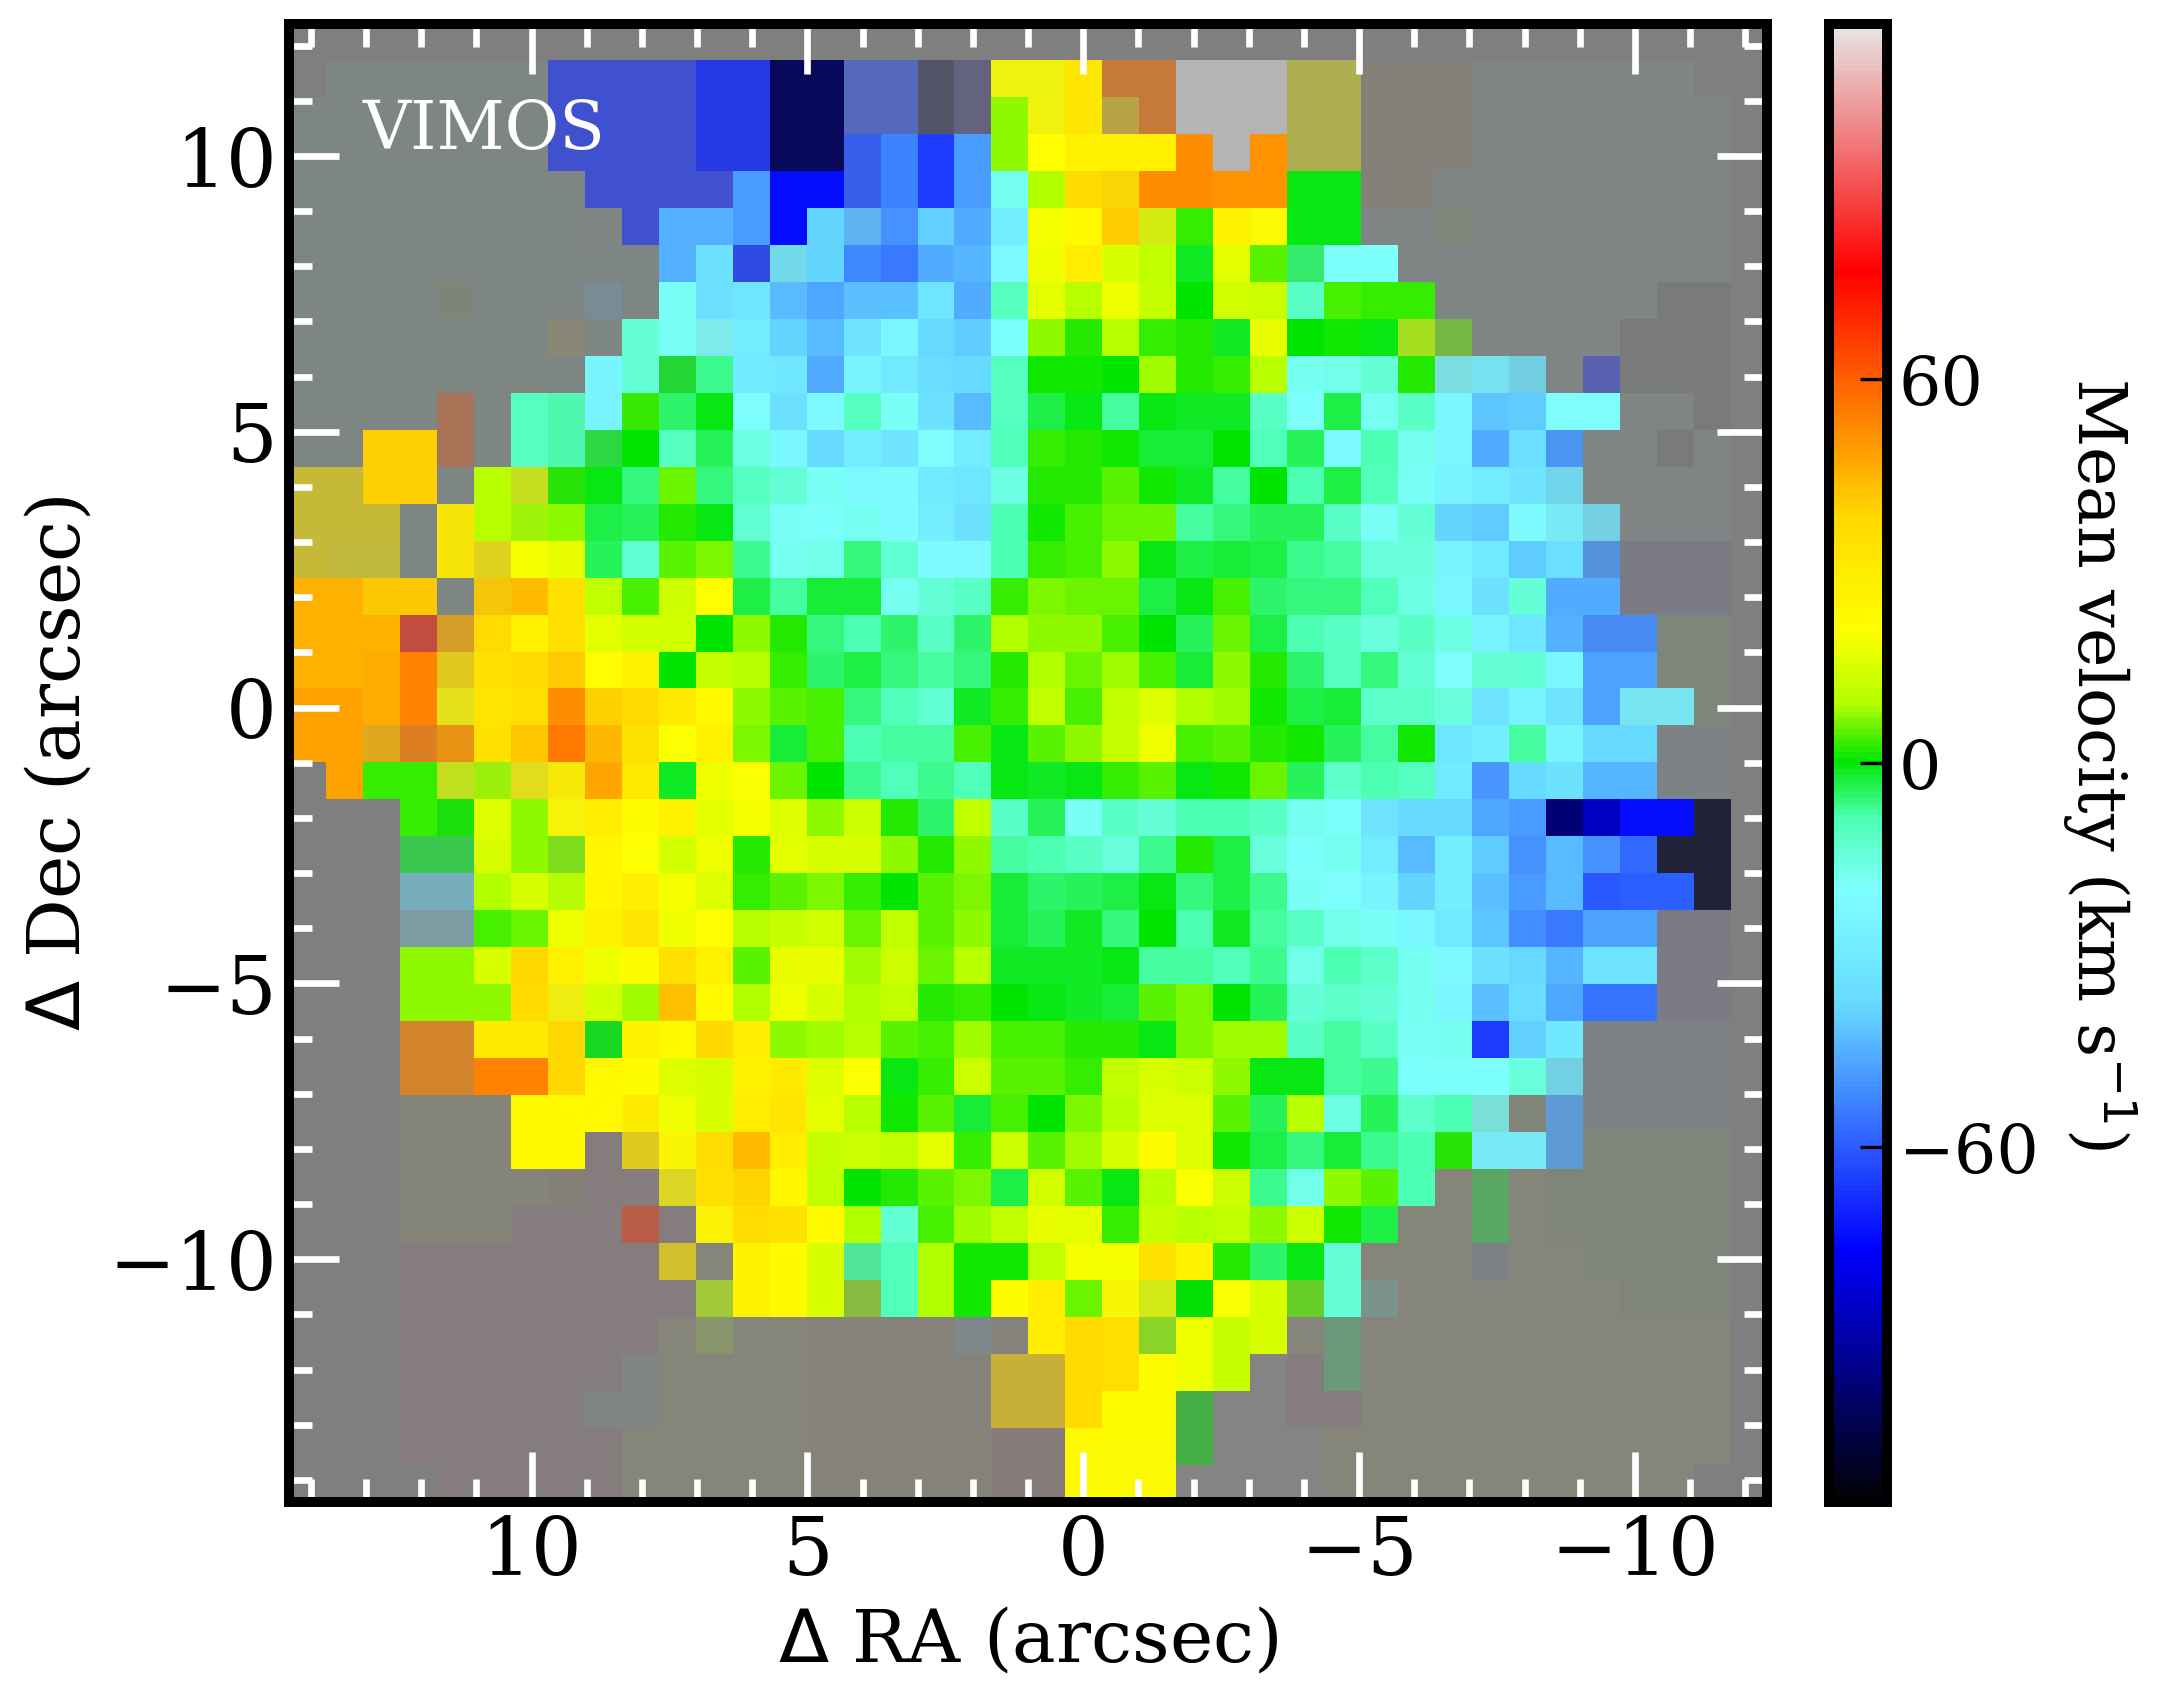
\includegraphics[width=.4\textwidth]{chapter2/VIMOS_NGC1399_vel.png}
			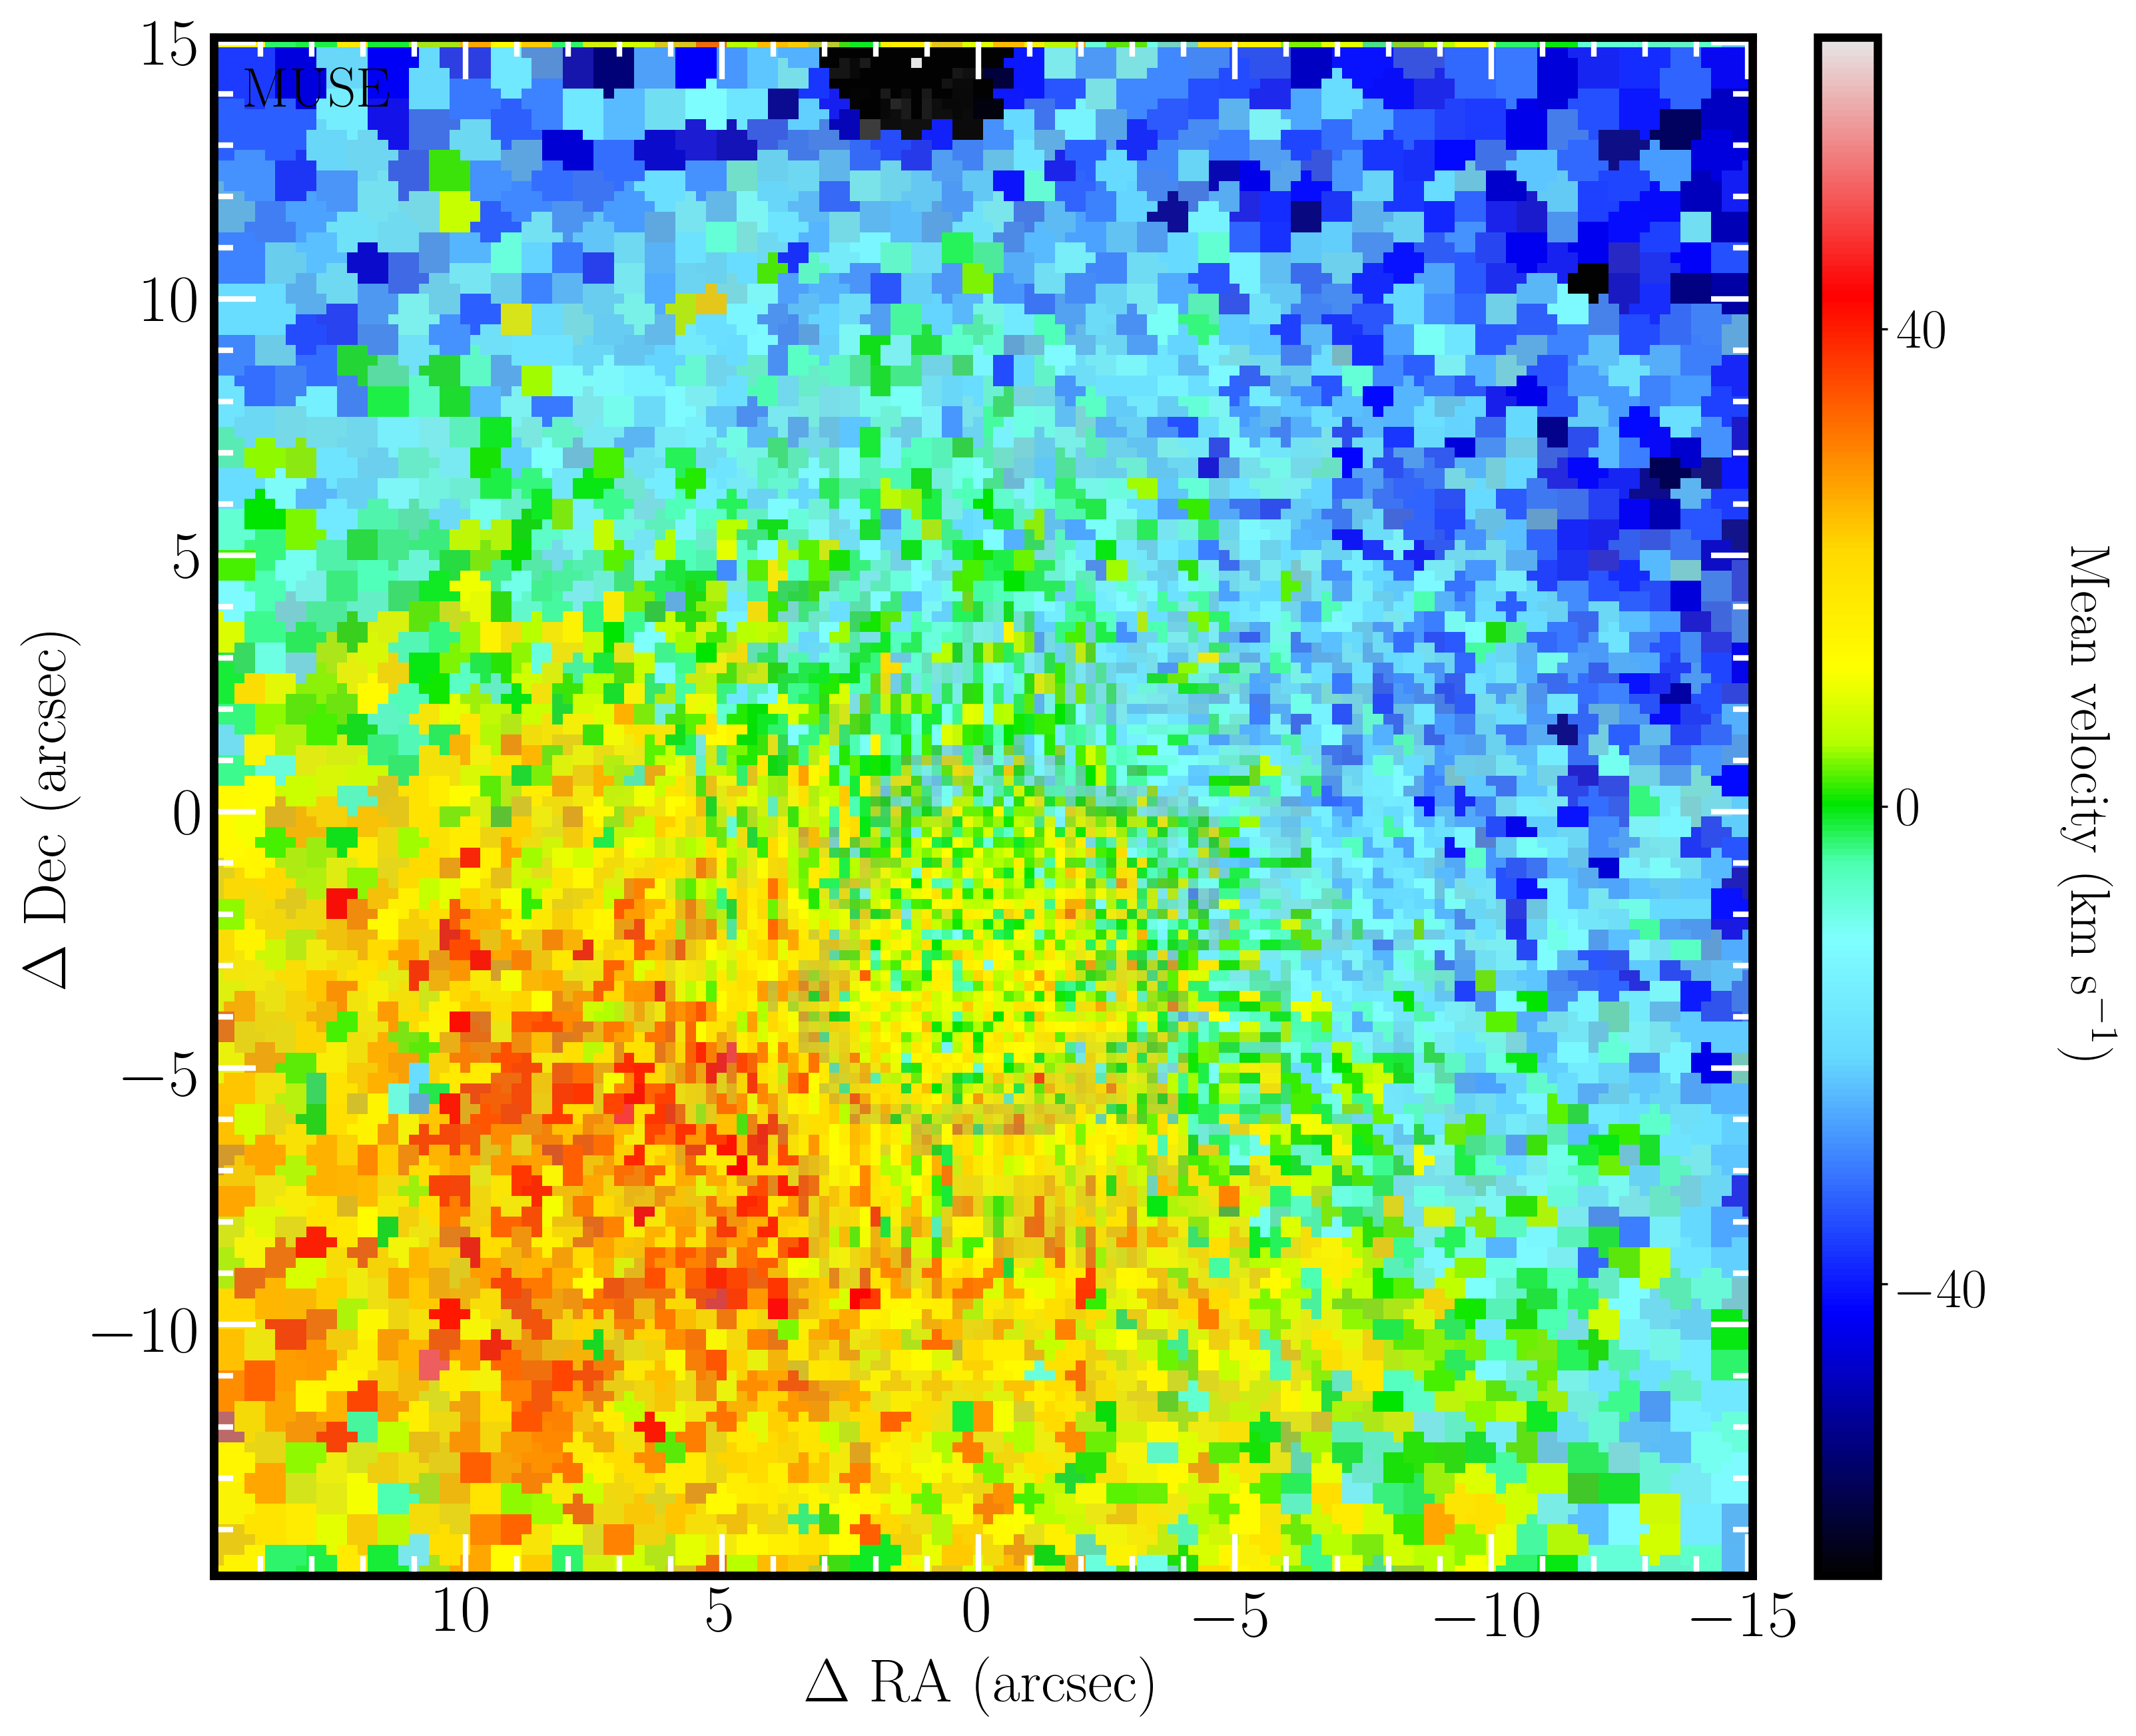
\includegraphics[width=.4\textwidth]{chapter2/MUSE_NGC1399_vel.png}
			\caption[Issues with wavelength calibrations in VIMOS data]{The mean velocity map for NGC 1399 demonstrating the offset in wavelength calibrations between the quadrants. Left panel: VIMOS map. Right panel: MUSE (see Section \ref{sec:MUSE}) map.}
			\label{fig:egVel}
		\end{figure}

		The ad-hoc corrections applied will correlate much of the data. However the affect should not be large and we therefore chose to neglect this correlation and treat these corrections as absolute i.e. the variance spectra are scaled by the same factor as the observed spectra. These correction will however, spatially smooth the data. This is particularly undesirable at the centres of our sample, where the affects of the active-galactic nuclei (AGN) should be observed. This should be taken into account (particularly for Chapter \ref{cha:Gas}).


	\subsection{Other Pipelines Tested}
		\label{subsec:Other}
		There are two other data-reduction pipelines that are publicly available. First is the ESO supplied VIMOS pipeline recipe (a plug-in) for their general purpose data handling tool \textsc{Gasgano}. At the start of this project, this pipeline was not well received by the community. Indeed ESO support suggested I try the alternative: \textsc{P3D}. Upgrades have since been made to both the instrument and the pipeline as well as improving the suggested observing schedules to remove some of the issues that we found when calibrating. 
		
		\textsc{P3D} is a comprehensive, multi-instrument package with both a decent graphical user interface (GUI) and an \textsc{IDL} application programing interface (API). It includes all the standard reduction steps: bias subtraction, tracing the fibre peak along the dispersion axis of the CCD, flat-fielding, wavelength calibration, flux calibration, cosmic-ray removal and DAR corrections. It also combined the quadrants into a single fits file, though as mentioned above, the calibration between the quadrants was attempted by comparing the relative intensities of the blended sky line at 5199\,\AA. This calibration step failed in most cases as the sky line is extremely faint (or non-existent) in many of the observations. As extremely sharp transitions were observed between the quadrants (See example in left panel of Fig.\,\ref{fig:P3D}). 

		\begin{figure}
			\centering
			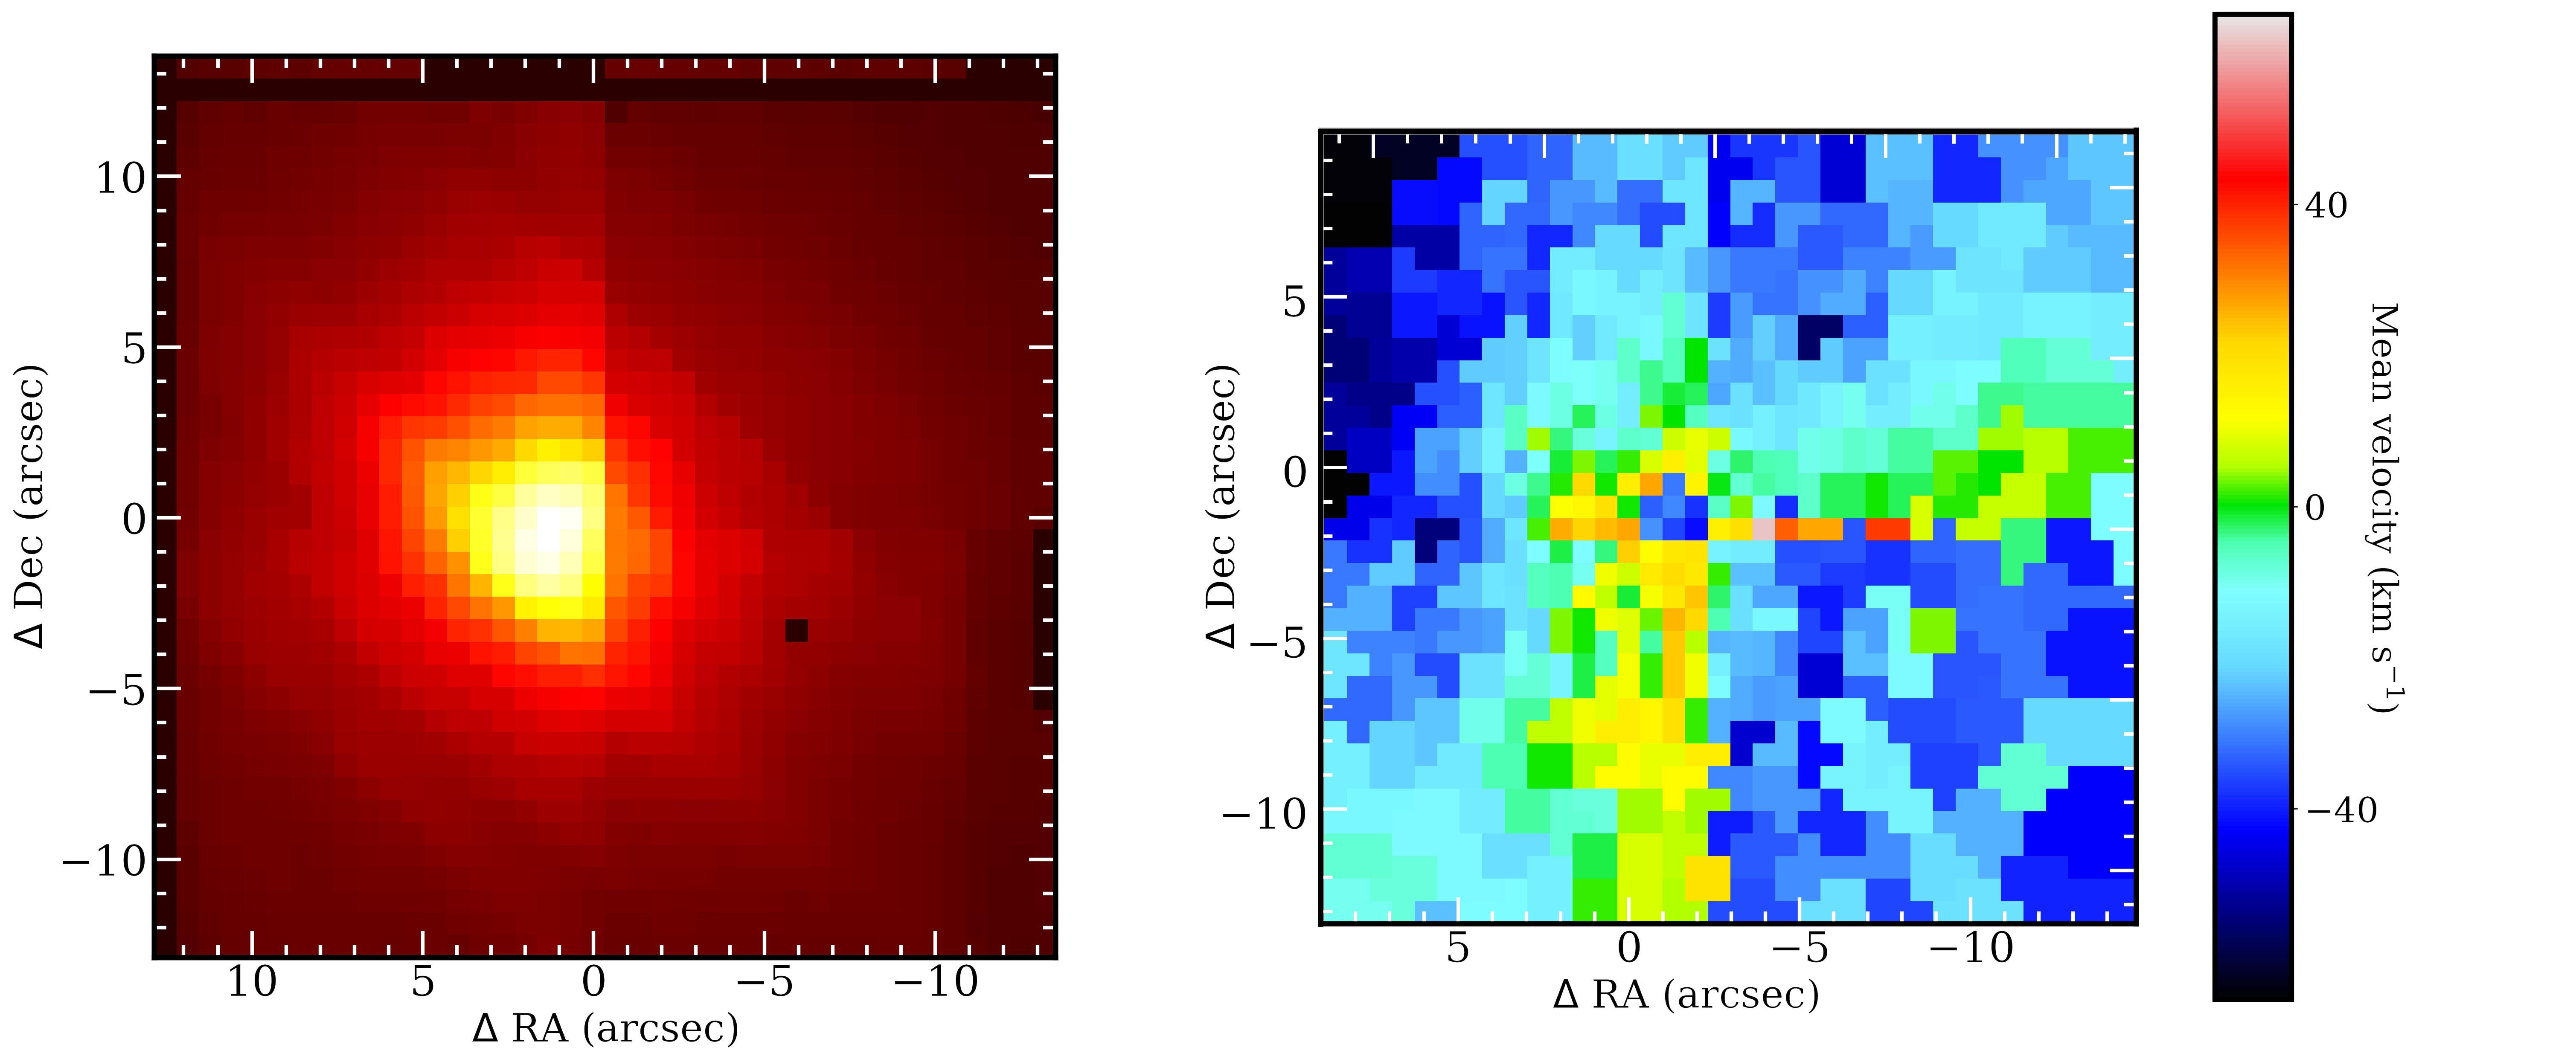
\includegraphics[width=.9\textwidth]{chapter2/P3D_NGC1399.png}
			\caption[Demonstrating issues with \textsc{P3D}-reduced data]{Examples of issues with \textsc{P3D}-reduced data for NGC 1399. Right panel: the flux map (image) Left panel: the mean velocity map. Both show sharp transitions between quadrants. The velocity map has had the outer 2 spaxels on all side discarded.}
			\label{fig:P3D}
		\end{figure}


		The wavelength-calibration step also was not very successful. Sharp transitions between the quadrants was also observed in an offset of the spectral direction. While this was still observed with \textsc{Py3D}-reduced data, the issue was much worse and more prevalent in \textsc{P3D}-reduced data. The right panel of Fig.\,\ref{fig:P3D} show the velocity map for NGC 1399 as an example of this issue in the \textsc{P3D}-reduced data. Here, the issue is so bad that rotation of the galaxy is completely .

		






\section{The Multi-Unit Spectroscopic Explorer (MUSE)}
	\label{sec:MUSE}
	\subsection{The MUSE Instrument}
		The Multi-Unit Spectroscopic Explorer (MUSE) is located on UT4 of the VLT. It is comprised of 24 IFU modules with a total field of view of 1 x 1' at spatial sampling of 0.2". It has a spectral range of 4800-9300\,\AA\ with a resolution of $\approx 2.3$\,\AA\ sampled at 1.25\,\AA\,pix$^{-1}$. MUSE is currently offered with and without adaptive optics (AO) and a narrow-field mode (with an order of magnitude between spatial resolution and sampling) is planned for the future. 
		
	\subsection{MUSE Archival Observations}
		Four of the sample (IC 1459, IC 1531, NGC 1316 and NGC 1399) where found to be in the archive of MUSE data.

		NGC 1316 (observed as part of Program ID: 094.B-0298A) and NGC 1399 (Program ID: 094.B-0903A) where both observed as mosaics, while IC 1459 and IC 4296 (both also Program ID: 094.B-0298A) where observed in single pointing. All were observed in the wide-field mode without adaptive optics in service mode during ESO period 94. 

		Every OB in both programs were observed following the standard MUSE calibration plan.

	\subsection{Reducing MUSE Data}
		For this project, the prereduced (known as Phase 3) data products from ESO were used. This means the ESO data reduction pipeline\footnote{http://www.eso.org/sci/software/pipelines/muse/muse-pipe-recipes.html} had already been applied. This was used since the computing resources required to reduce the raw MUSE data may have been prohibitively large.

		The ESO pipeline contains all standard IFU data reduction steps: bias subtraction, flat-fielding of detectors with a continuum lamp exposure, flat-fielding of fibres with twilight exposures, wavelength calibration, flux calibration with standard star observations and sky subtraction. Tiled observations, where present, are combined to give a final mosaic.

		We found that the Phase 3 data products were generally of a sufficient quality for our purposes, except that the sky subtraction in both IC 1459 and IC 426 appear to have over-subtracted large portions of the spectra. This gave the impression of enormous absorption features (often with negative fluxes). To remove this over-subtraction, our own pseudo-sky subtraction routine was developed. The median spectrum was taken from four 20 x 20 spaxel boxes taken from each corner of the observation. After checking that no stellar continuum could be fitted to the spectrum (i.e. that very little light from the galaxy was contaminating our pseudo-sky spectrum), this spectrum was subtracted from each spaxel in the cube. 

		Extra (pseudo-) sky subtractions for NGC 1316 and NGC 1399 were not possible due to mosaic nature of the observations since a sky subtraction should to be applied to each observation in the mosaic independently. The observations are already combined as part of the automated data reduction. It is also not possible to access data products from part way through the data reduction, such as immediately before the mosaic is produced. Both NGC 1316 and NGC 1399 are not as badly affected as IC 1459 and IC 4296, so they are left uncorrected. 

		Finally, we trimmed all the cubes to the central 30" x 30" (150 x 150 spaxels) in order to (a) avoid the region used for the pseudo-sky spectrum and (b) reduce the computing resources required for the spatial binning stage in the data analysis (Section \ref{sec:analysis}). 

		As with the VIMOS data, the variance is propagated throughout the entire data reduction pipeline and is squared-rooted here to be used as the noise input in the analysis stage. 
\section{Data Analysis}
	\label{sec:analysis}
	From this point on, the two datasets are treated almost identically. The only difference (other than the different spectral range and resolutions) is that the MUSE datacubes were binned to a higher signal to noise ratio (S/N).

	The entire pipeline is summed up as follows.
	\begin{enumerate}
		\item Spatially bin using Voronoi binning.
		\item Find the relevant stellar templates by fitting the entire galaxy spectra with all the templates from the Miles library and using only the non-zero weighted templates from this step from here on in.
		\item Estimate redshifts and global line-of-sight velocity dispersion with MCMC routine. 
		\item Find the best-fitting LOSVD for the stellar and emission line components for each individual bin. A bootstrapping method to estimate uncertainties LOSVD measurements. 
		\item Removing the fitted emission lines from the previous step, measure absorption line strengths. 
		\item Finally, use these absorption line strengths to find the best-fitting stellar population models.
	\end{enumerate}


	\subsection{Spatial Binning}
		\label{subsec:Binning}
		Given that galaxies (the signal) are brightest at the centre and fades away radially, and noise, which is assumed to be Poisson dominated, scales as the square root of the signal, the S/N will also be highest at the centre, decreasing with increasing radius. In the outer regions of a galaxy, it becomes too low for to make meaningful fits to the spectra. Because of this we spatially bin to a fixed S/N (increasing a bins size until it reaches the required S/N). This is performed using a Voronoi Binning routine\footnote{http://www-astro.physics.ox.ac.uk/~mxc/software/} by \citet{Cappellari2003}. To do this, we defined `signal' and `noise' as the median value of the spectrum and noise spectrum respectively for each spaxel. A S/N of 30 is required for all VIMOS datacubes and 50 for IC 1459 and IC 4296 MUSE datacubes. NGC 1316 and NGC 1399 MUSE datacubes were binned to a S/N of 50 for analysis of the stellar kinematics and 100 for analysis of the emission line kinematics and stellar population. The MUSE datacubes had differing S/N due to the extra (pseudo-)sky subtractions which were applied to IC 1459 and IC 4296. These sky subtractions were successful in removing artifacts from the spectra, allowing us to retain a higher level of spatial information for these two galaxies. The artifacts did not seem to affect the analysis of the stellar kinematics, but did affect the emission line fitting. For this reason we enforced a higher S/N for analysis of the emission lines and where careful subtraction of the emission lines is important (i.e. in analysis of the stellar populations). Figure \ref{fig:egSNR} shows an example of the S/N of the bins. In it, concentric ringed structures can be clearly seen around the centre of the galaxy as bins with a S/N just below the target are increased in size by a single spaxel. This means they have a final S/N well over the target.

		\begin{figure}
			\centering
			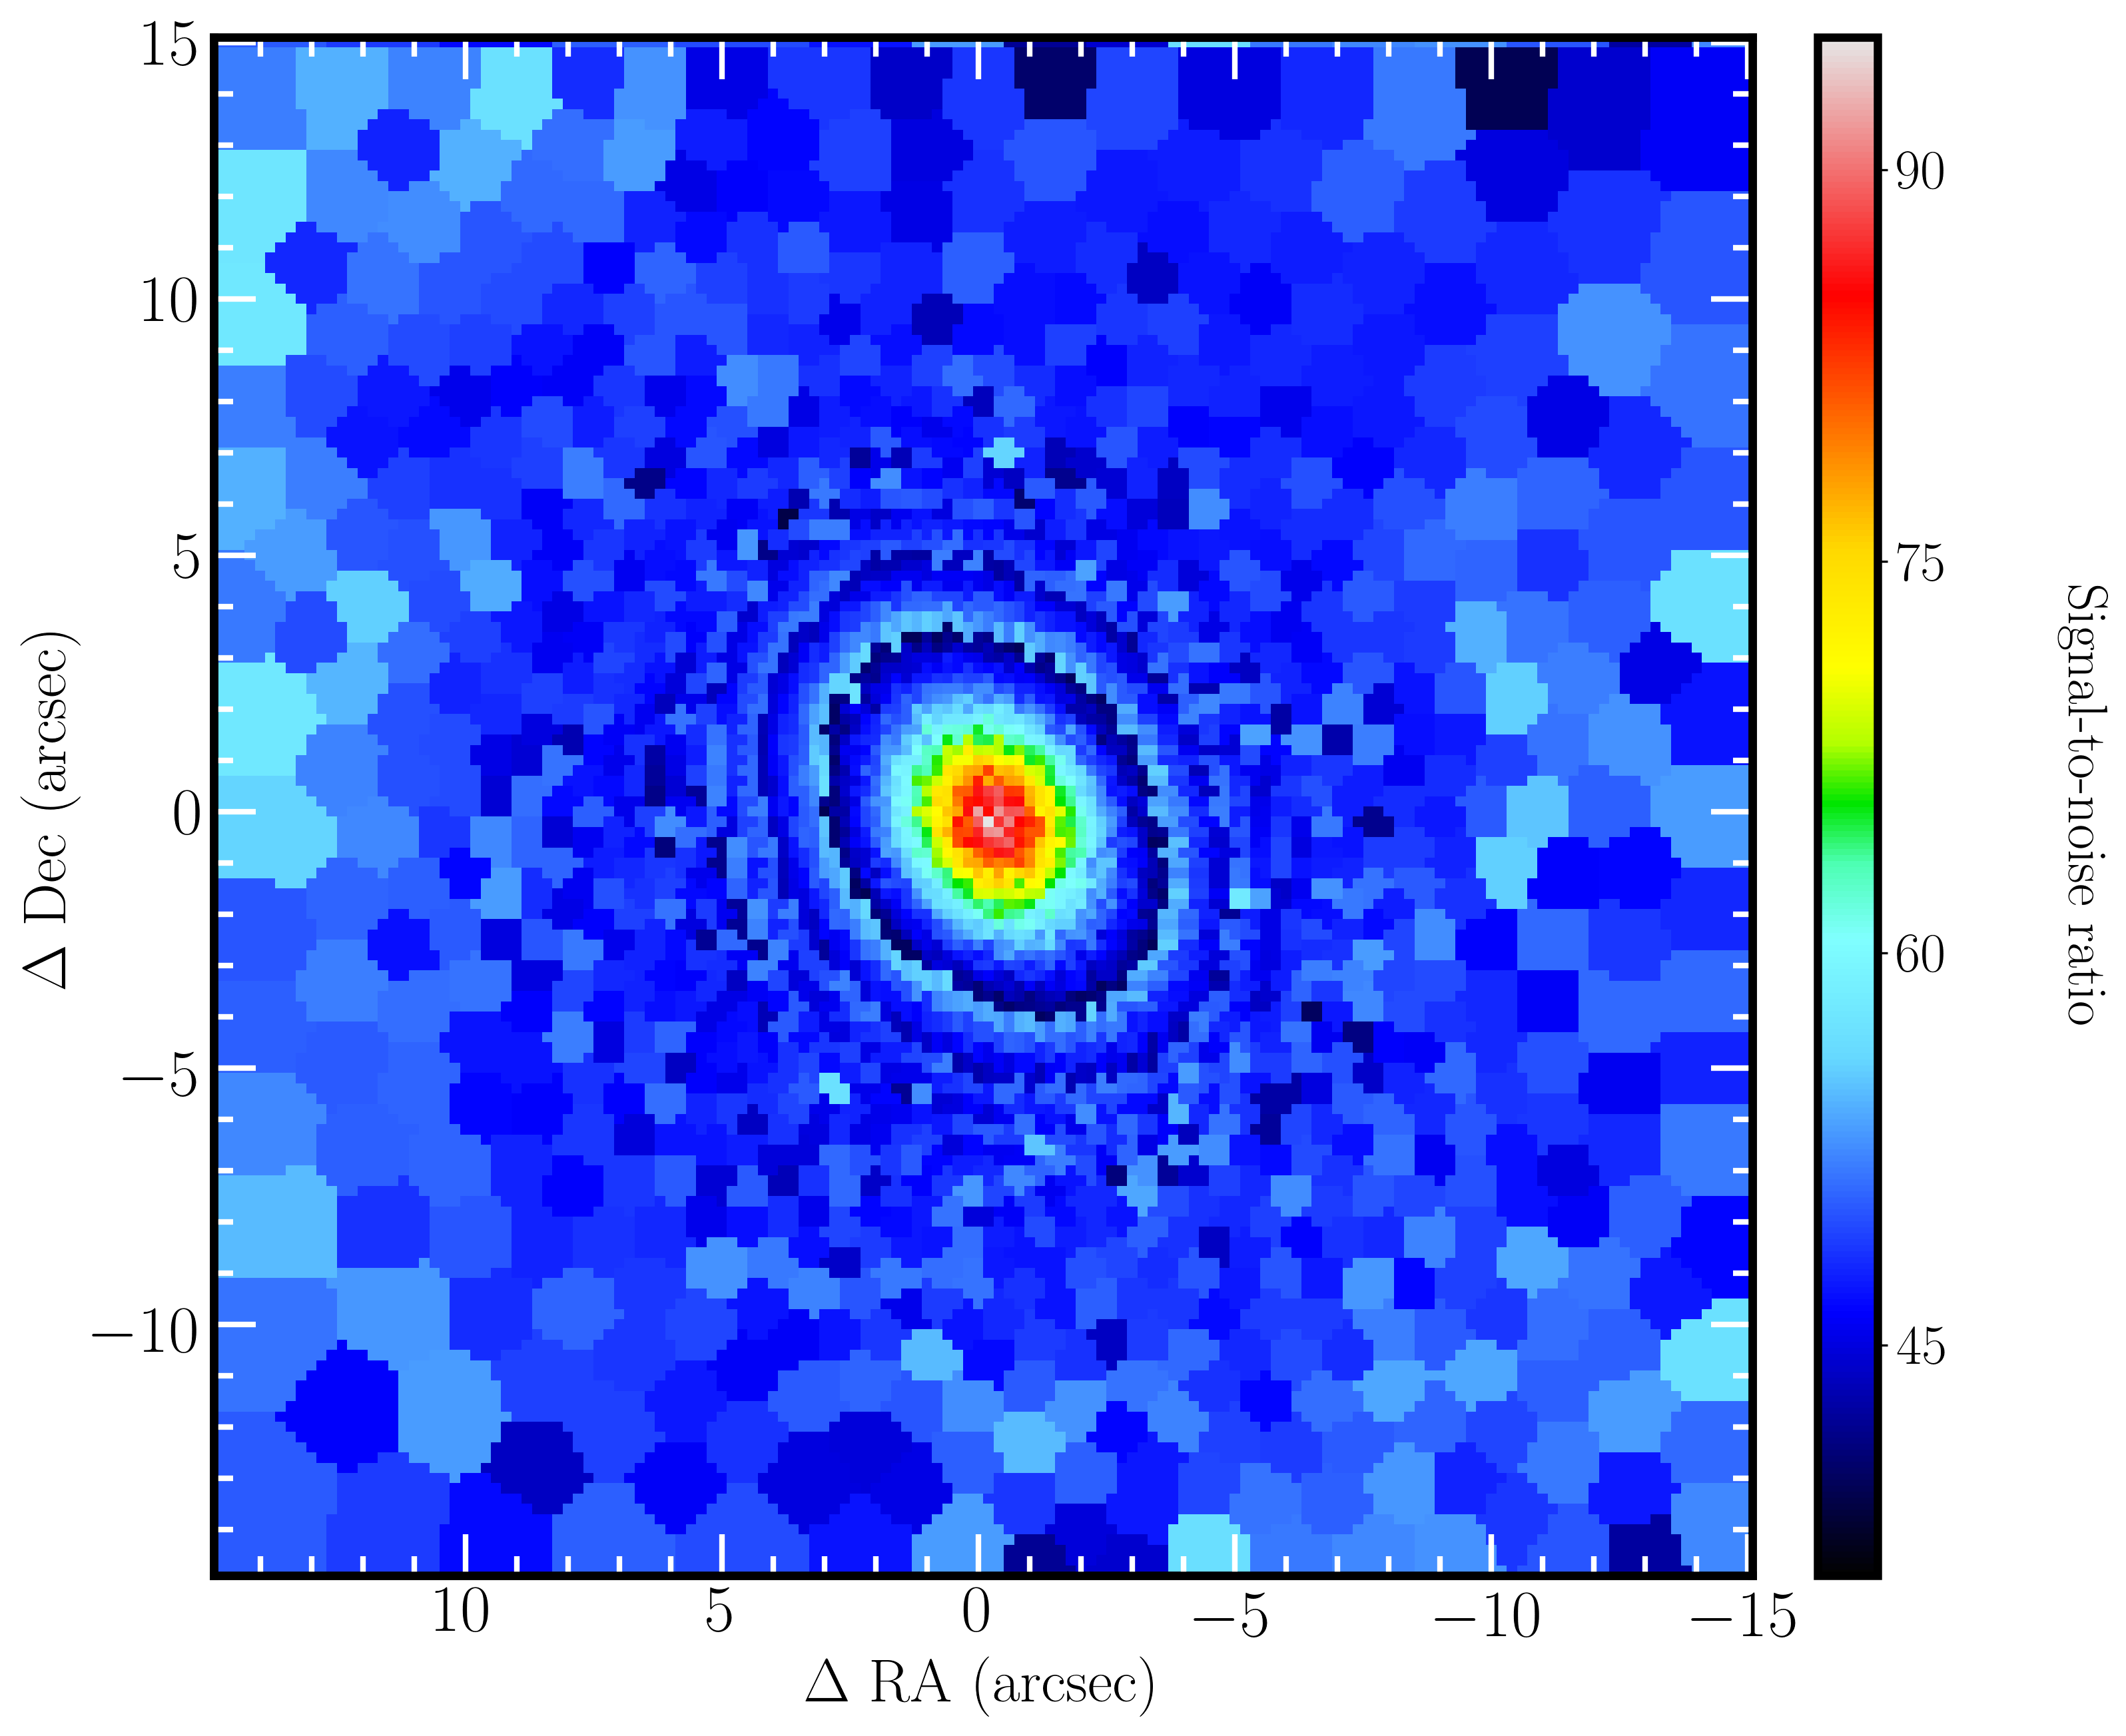
\includegraphics[width=.6\textwidth]{chapter2/egSNR.png}
			\caption[Example S/N map]{The figure shows an example S/N map for the MUSE observation of IC 1459.}
			\label{fig:egSNR}
		\end{figure}

	\subsection{Stellar Kinematics}
		\label{subsec:StellarFit}
		Our analysis makes use of the penalized-fitting routine \textsc{pPXF}\footnote{http://www-astro.physics.ox.ac.uk/~mxc/software/} by \citet{Cappellari2004, Cappellari2016a}. This routine finds the best-fitting kinematics by minimizing the reduced chi-squared of a fitted spectrum built from combined empirical stellar templates, convolved with a Gaussian line-of-sight velocity distribution (LOSVD; here parametrised by the mean velocity, $v$, and velocity dispersion, $\sigma$, only). Gaussian templates can also be used to fit emission lines from the interstellar medium (ISM) as independent components (with their own LOSVD). \textsc{pPXF} requires an initial guess for the LOSVD for each component. We use the redshift of the galaxy and $200\,\mathrm{km\,s^{-1}}$ for the initial velocity and velocity dispersion estimates. Finally, Lagrange polynomials can be used to make additive or multiplicative corrections to the continuum level of the fit. A possible sky line at 5199\,\AA\ in the Earth's frame of reference is masked in all fits.

		In order to improve the speed of our analysis, we first collapse the datacube spatially to give a global spectra for the galaxy by summing across both spatial dimensions at each wavelength. Then the entire Miles stellar library \citep{Sanchez-Blazquez2006, Falcon-Barroso2011a} is used as templates for \textsc{pPXF} to fit. $600\,\mathrm{km\,s^{-1}}$ wide regions around possible emission lines (see Table \ref{tab:EmissionLine}) are masked and a fourth order Lagrange polynomial is used for an additive continuum correction. We use the redshift values from Simbad \citep{Wenger2000} for our initial velocity estimate. For our 14 datacubes (10 VIMOS and 4 MUSE), this step fits an average of 23 templates out of 985 with a non-zero weighting. Zero-weighted templates are discarded in future analysis of a given datacube. This drastically improves the runtime of \textsc{pPXF} without effecting the quality of the fit.

		% For this fit the redshift from Simbad is used to move the spectra to the rest frame such that an initial guess of the velocity within that frame is 0 km s$^{-1}$. We use a initial guess of the velocity dispersion of 200 km s$^{-1}$ since ETGs have dispersions of around this value and higher. 



		%Regions (600 km s$^-1$ wide) around possible emission lines were masked. Emission lines included were: [OII]3726 , [OII]3729, H$_\delta$, H$_\gamma$, H$_\beta$, [OIII]4959, [OIII]5007, [NI]5199, [NI]5202, [OI]6300, [OI]6364, [NII]6548, [NII]6583, H$_\alpha$, [SII]6716 and [SII]6731. A telluric line at 5199 \AA, seen in some of the VIMOS spectra, was also masked, though the exact location of this depended on the initial redshift 'guess' since the spectrum is moved to the rest frame of the galaxy. For this analysis, we also allowed an additive continuum correction using a fourth order Lagrange polynomial.

		Next we run a Markov chain Monte Carlo (MCMC) routine to find more optimum initial estimates for velocity and velocity dispersion. For each observation, the initial run is set up in the same way as the previous step (though only using the templates with non-zero weightings). After each run, the fitted velocity and velocity dispersion are used as the initial estimate for \textsc{pPXF}, thus iteratively improving the initial guess with each subsequent run. After the first three repetitions, the velocity was used to calculate the precise redshift of the galaxy: these are the redshift values quoted in \ref{tab:sample}. After this, small random perturbations to the iterative initial estimates are applied to ensure that the routine converges on a global minimum chi-squared, rather than a local one. 100 repetitions are run, with the mean velocities and velocity dispersions recorded and used as the initial estimates for all subsequent fits in that datacube. 

		Beyond this point, each bin is analyzed independently. Each one is processed through \textsc{pPXF} using only the Miles templates with non-zero weighting from above, using the redshift, additional velocity and dispersion estimates from the last step as the initial required estimate. Again regions around emission lines are masked, and a fourth order additive continuum correction is used. To allow accurate estimation of the propagation of uncertainties in the best-fitting values, a bootstrapping method with 1000 repetitions is used. In each iteration (after the first), random noise, distributed with a Gaussian profile and an amplitude comparable to the noise propagated through the data reduction pipeline, is added to the best-fitting spectrum from the first run. The standard distribution of the fitted parameters from each iteration is used as the quoted uncertainty.


	\subsection{Emission-line Kinematics}
		\label{subsec:EmissionFit}
		Fitting emission lines is achieved in a similar fashion to finding the stellar kinematics. However, in order to combat template mismatches, where emission lines are erroneously fitted to the edges of absorption features that are under represented bu the stellar templates, we follow the method set out in \citet{Sarzi2005}. This is a three step process.
		\begin{enumerate}
			\item The region around each emission line's rest frame wavelength is masked, and the stellar spectrum is fitted.
			\item The kinematics of the stellar spectrum is fixed to the kinematics found in step 1. The region around the [\ion{O}{iii}] doublet is then unmasked and fitted.  
			\item All emission lines are unmasked, but have their kinematics fixed to that found for [\ion{O}{iii}] in Step 2. The emission lines are therefore being fitted with their amplitudes as their only free parameter. 
		\end{enumerate}
		All steps are repeated with the MC method described above to propagate uncertainties and include a tenth order multiplicative Lagrange polynomial to account for continuum emission. 

		The residuals between the best-fitting spectra and the input spectra are smoothed and averaged using a weighted, moving average. This is then summed in quadrature with the noise spectrum to give a combined `residual noise' spectrum. For each fitted emission line, $i$, the amplitude (of the fitted line) to the median residual noise (in the region of the emission line) ratio $(A/N)_i$. is used as a detection threshold. As in \citet{Sarzi2005}, a fit for [\ion{O}{iii}] only is considered a detection if $(A/N)_{[\text{\ion{O}{iii}}]} \ge 4$. For all other lines, $i$, except [\ion{N}{i}], a detection is recorded if [\ion{O}{iii}] is detected in the same bin and $(A/N)_\mathrm{i} \ge 3$; while a detection of [\ion{N}{i}] requires a detection of both [\ion{O}{iii}] and H\,$\beta$ and $(A/N)_{[\text{\ion{N}{i}}]} \ge 4$. Emission lines included are given in Table \ref{tab:EmissionLine} along with their rest wavelengths and that of any doublet counterparts (for so-called forbidden lines). 

	 	\begin{table}
	 		\centering
	 	\begin{threeparttable}
	 		\caption{Emission lines included in \textsc{pPXF} fit.}
	 		\label{tab:EmissionLine}
	 		\begin{tabular}{l c c}
	 		\hline
	 		\hline
	 		Line name 		& Emission line & Doublet counterpart  \\
	 		 & rest-frame wavelength (\AA) & wavelength (\AA) \\
	 		\hline
	 		\bracket{\ion{O}{ii}} 	& 3726.03 & 3728.82 \\
	 		H\,$\delta$ 	& 4101.76 \\
	 		H\,$\gamma$ 	& 4340.47 \\
	 		H\,$\beta$ 		& 4861.33 \\
	 		\bracket{\ion{O}{iii}}	& 4958.92 & 5006.84 \\
	 		\bracket{\ion{N}{i}} 	& 5199.36 & 5201.86 \\
	 		\bracket{\ion{O}{i}} 	& 6300.30 & 6363.67 \\
	 		\bracket{\ion{N}{ii}} 	& 6548.03 & 6583.41 \\
	 		H\,$\alpha$ 	& 6562.30 \\
	 		\bracket{\ion{S}{ii}} 	& 6716.47 & 6730.85 \\
	 		\hline
	 		\hline
	 		\end{tabular}
	 	\end{threeparttable}
	 	\end{table}




	 \subsection{Stellar Populations}
	 	\label{subsec:PopFit}
	 	In order to investigate the stellar populations of our sample we assume that a given spectra (a global, spatially integrated spectrum or the spectrum from a given bin) is well approximated to a simple/single stellar population (SSP), i.e. that spectrum represents a system of stars all born at the same time, in the same environment. 

	 	There are two methods for finding the best-fitting SSP: full spectral fitting of synthetic spectra with different properties or compare the observed absorption line strengths to empirical or modeled line strengths. The former has the advantage of retaining more information, being able to fit fine structure in the spectrum and can easily find complex stellar populations. It does, however, rely on highly reliable synthetic spectra for each permutation of stellar population properties that is considered. Also, for massive ETGs, fine structures in spectra are lost because of the smoothing from the high velocity dispersions. 

	 	The latter has the advantage of only considering the parts of the spectrum that are highly sensitive to the stellar population. It can be more easily based on empirical observations of stars in the solar neighborhood and thus is less model dependent. Interpolation between well populated regions of the parameter space of the stellar population properties can be used to minimize the errors in sparse regions of the parameter space. We also found that full spectral fitting almost always returned models from an extreme corner of the parameter space of models. For these reasons we use the absorption line strength approach.

	 	\subsubsection{Absorption Line Strengths}
	 		\label{subsubsec:Absorption}
	 		Absorption line strengths are measured as an equivalent width of a given index. Each index consists of 3 bandpasses: one blue and one red continuum bandpass on either side of the central bandpass containing the absorption feature. A pseudo-continuum is defined as a straight line between two points at the centre of each continuum bandpass with heights of the median intensity of the given bandpass. The index, $I$, is measured as the equivalent width of the spectrum, $F_\mathrM{I}(\lambda)$, within the central bandpass (defined between wavelengths $\lambda_1$ and $\lambda_2$) with respect to this pseudo-continuum, $F_\mathrm{C}(\lambda)$, i.e for the so-called atomic indices, measured in \AA,
	 		\begin{align}
	 			I_\text{\AA} \equiv \, & \int^{\lambda_2}_{\lambda_1} \! \left(1 - \frac{F_\mathrm{I}(\lambda)}{F_\mathrm{C}(\lambda)}\right) \, \mathrm{d}\lambda \, , \\
	 		\intertext{while molecular indices, measured in magnitude units is}
	 			I_\text{mag} \equiv \, & -2.5 \log\left(\frac{1}{\lambda_2 - \lambda_1} \int^{\lambda_2}_{\lambda_1} \! \frac{F_\mathrm{I}(\lambda)}{F_\mathrm{C}(\lambda)} \, \mathrm{d}\lambda\right) \, .
	 		\end{align}
	 		The indices we use for this project, along the defining bandpasses are taken from \citet{Trager1998} and are given in Table \ref{tab:abIndex}.


		 	\begin{table}
				\centering
			\begin{threeparttable}
				\caption{Definitions of bandpasses for line indices.}
				\label{tab:abIndex}
				\begin{tabular}{l c c c}
					\hline
					\hline
					Index 	& Blue cont. 		& Index band 		& Red cont. \\
					\hline 
					G4300 	& 4266.375--4282.625 & 4281.375--4316.375 & 4318.875--4335.125 \\
					Fe4383 	& 4359.125--4370.375 & 4369.125--4420.375 & 4442.875--4455.375 \\
					Ca4455 	& 4445.875--4454.625 & 4452.125--4474.625 & 4477.125--4492.125 \\
					Fe4531 	& 4504.250--4514.250 & 4514.250--4559.250 & 4560.500--4579.250 \\
					H\,$\beta$ & 4827.875--4847.875 & 4847.875--4876.625 & 4876.625--4891.625 \\
					Fe5015 	& 4946.500--4977.750 & 4977.750--5054.000 & 5054.000--5065.250 \\
					Mg\,b 	& 5142.625--5161.375 & 5160.125--5192.625 & 5191.375--5206.375 \\
					Fe5270 	& 5233.150--5248.150 & 5245.650--5285.650 & 5285.650--5318.150 \\
					Fe5335 	& 5304.625--5315.875 & 5312.125--5352.125 & 5353.375--5363.375 \\
					Fe5406 	& 5376.250--5387.500 & 5387.500--5415.000 & 5415.000--5425.000 \\
					Fe5709 	& 5672.875--5696.625 & 5696.625--5720.375 & 5722.875--5736.625 \\
					Fe5782 	& 5765.375--5775.375 & 5776.625--5796.625 & 5797.875--5811.625 \\
					NaD 	& 5860.625--5875.625 & 5876.875--5909.375 & 5922.125--5948.125 \\
					TiO1 	& 5816.625--5849.125 & 5936.625--5994.125 & 6038.625--6103.625 \\
					TiO2 	& 6066.625--6141.625 & 6189.625--6272.125 & 6372.625--6415.125 \\
					\hline
					\hline
				\end{tabular}
				\begin{tablenotes}
				\footnotesize
				\item \textit{Notes:} Indices are from \citet{Trager1998}.
				\end{tablenotes}
			\end{threeparttable}
			\end{table}

			Much of the literature measures absorption line strengths under the Lick/Cassegrain image dissector scanner spectrograph system (hereafter Lick/IDS system; \citealt{Faber1985, Worthey1994}). This has several disadvantages. Firstly, the Lick/IDS system is based on non-flux calibrated spectra from the IDS spectrograph on the Shane telescope (Lick Observatory), which has a relatively low and wavelength-dependent spectral resolution. When using the Lick/IDS system with other instruments, it is thus necessary to calibrate the observations by performing empirical corrections to correct for the uncalibrated continuum of the Lick/IDS data. This requires observations of standard stars with the same instrumental set-up as the main observations. Since this was not requested as part of the VIMOS observing strategy, we are not able to do this (a later proposal was not possible either as VIMOS was substantially upgraded in the intervening time). Given the low spectral resolution and poor data quality on which the Lick/IDS system is based, we believe in any case that the community should be making a concerted effort to use alternative systems. We therefore choose to use an alternative: the line index system (LIS) of \citet{Vazdekis2010}. LIS is based on flux calibrated measurements as several resolutions (5.0, 8.4 and 14.0\,\AA). \citet{Vazdekis2010} also provide empirical cubic functions for transforming literature measurements from the Lick/IDS system to LIS\footnote{http://www.iac.es/proyecto/miles/pages/line-index-system-lis/transformations.php}.

			Because of the models we use for stellar population fitting (detailed in Section \ref{subsubsec:StellarPop}), we actually measure absorption indices at a resolution of 2.5\,\AA\ (FWHM). For the purposes of comparisons to the literature (see Section \ref{subsec:absorption}) we also measure the absorption indices at 8.4\,\AA\ resolution. 

			Since the aim is to find the best-fitting stellar population is it important that we first remove the effect of the ISM. This involves fitting for (as described in Section \ref{subsec:EmissionFit}) and subtracting detected emission lines. 

			We must also correct for the effect of velocity dispersion of the stellar populations which will spread absorption features such that some of the absorption is outside of the central bandpass. To do this, we first build a spectrum that is not convolved with the velocity dispersion. This is done by creating the best-fitting spectrum (as in the previous step), but not convolving it with the LOSVD. A given index, $i$, is measured for both this `unconvolved' spectrum, ($I^\text{unc}_i$) and the convolved best-fitting spectrum ($I^\text{conv}_i$). The ratio of the indices measured for these two spectra is used as a (multiplicative) correction factor for the index measured on the emission line-corrected observed spectra ($I^\text{obs}_i$), such that
			\begin{equation}
				I^\text{corr}_i \equiv \frac{I^\text{unc}_i}{I^\text{conv}_i} I^\text{obs}_i \, .
			\end{equation}}


		\subsubsection{Fitting Stellar Population Models}
			\label{subsubsec:StellarPop}
			The final step of the data analysis pipeline is to find the best-fitting SSP models for a given spectrum. Sets of SSP models consist of a grid of models characterised by stellar properties such as age ($t$), metallicity ($[Fe/H]$) and alpha-element enhancement ($\alpha$-enhancement; $[\alpha/Fe]$). Here, we first give an overview of the process of generating synthetic stellar populations before detailing the specifics of the models used below. 

			Synthetic SSPs are created using the following components:
			\begin{itemize}
				\item the loci of a star of a given mass and metallicity, as they travel across the Hertzsprung--Russel Diagram (HRD) by aging. These are known as stellar evolutionary tracks and are generally empirical.
				\item the function, $\Phi(M)$, representing the number of stars formed, $N(M)$, for a given mass, $M$, respect to mass. I.e. $\Phi(M) \equiv \frac{\mathrm{d}N(M)}{\mathrm{d}M}$. This is the initial mass function (IMF).
				\item an empirical library of stellar spectra to be able to assign a a spectra to a position on the HRD. 
			\end{itemize}
			The desired output of expected line strengths for a 3 dimensional grid of varying age, metallicity and $\alpha$-enhancement can be computed in one of two ways: (i) producing full synthetic spectra from the evolution of stellar atmospheres or (ii) finding a `fitting function' for each index which analytically calibrates the line strengths measured from empirical libraries to physical stellar parameters. The former is dependent on a good understanding of the physics of stellar atmospheres and is known to suffer from incomplete line lists and continuum uncertainties \citep{Thomas2004}. This would have been the appropriate method for producing spectra for full-spectral fitting had we chosen that method for investigating stellar populations (see Section \ref{subsec:PopFit}). The latter, and more popular method, interpolates between well populated regions of the parameter space. This allows the computing of the uncertainties in the model predictions and decreases those uncertainties in sparse regions of the parameter space. 

			ETGs often have very different fractional abundances of various metals to the nearby stars that we are able to observe (all of which have near solar abundances). As such, the stellar libraries that are used to calibrate the models fall short of the required coverage of the parameter space. Most methods make some effort to extrapolate to non-solar abundances. In a similar way to the fitting functions described above, `index response functions' can be found. This calibrates the effect of varying abundances of individual elements. In this case, comparison must be made to completely theoretical spectra.

			We use the SSP models by \citet{Thomas2010} (referred to hereafter as the TMJ models) as they are based on flux calibrated spectra and therefore do not require calibration to the Lick/IDS system. These models assume a \citet{Salpeter1955} IMF ($\Phi(M) \propto M^{-2.35}$) and are based on the evolutionary population synthesis code by \citet{Maraston1998}. The models use stellar evolutionary tracks by \citet{Cassisi1997} for metallicities of $[Z/H] < -0.33$ and \citet{Girardi2000} for $[Z/H] \ge -0.33$; the MILES stellar spectral library by \citet{Sanchez-Blazquez2006a} and \citet{Falcon-Barroso2011a}; fitting functions by \citet{Johansson2010} and index response functions by \citet{Korn2005}. The MILES library gives the models a resolution of 2.5\,\AA\ (FWHM). This is below the resolution of the reduced VIMOS data (at 3\,\AA), but we in Fig.\,\ref{fig:res} we show that this effect is negligible. Comparing the absorption line strengths measured at 2.5\,\AA\ and 3\,\AA\ for the MUSE datasets shows the most effected index is Fe5782 with a mean difference of 1\% between the index measured at 3\,\AA\ and 2.5\,\AA. All other indices show a few tenths of a percent difference. 

			\begin{figure}
				\centering
				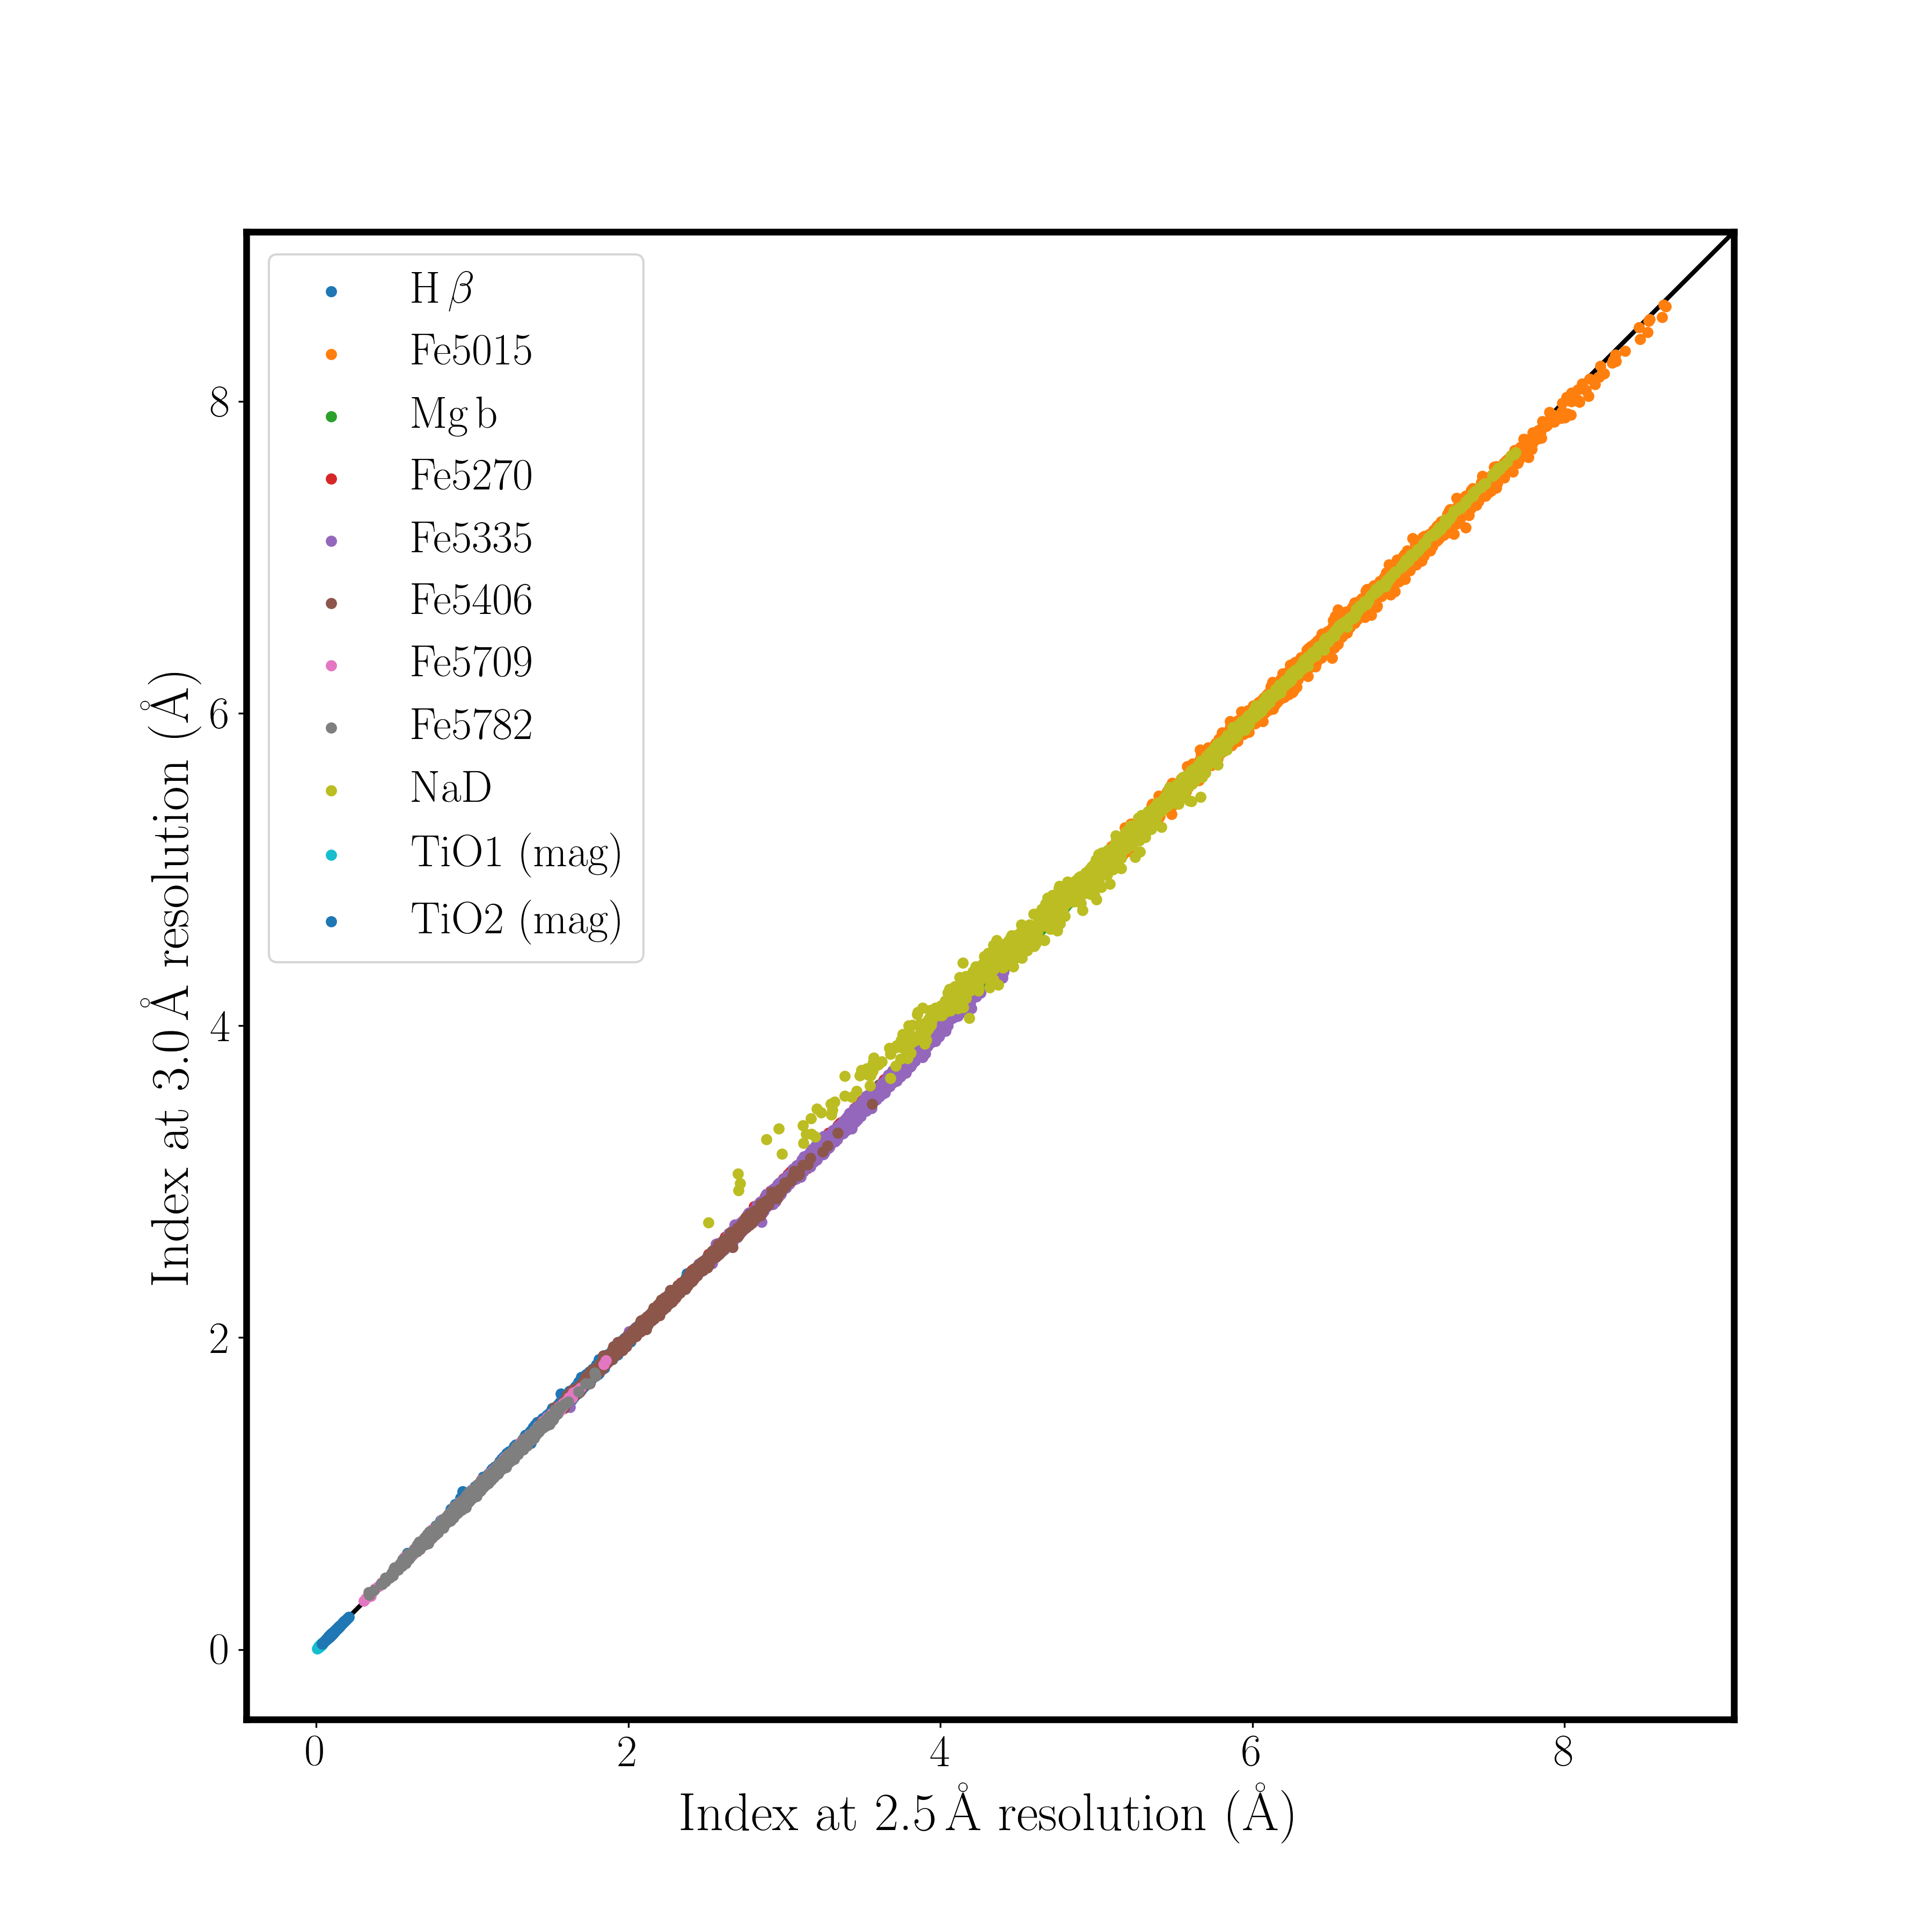
\includegraphics[width=.7\textwidth]{chapter2/compare_resolutions.png}
				\caption[Affect of resolution on absorption line index strength]{The effect of resolution of the measure absorption line strength. This shows that we can assume the effect of a lower spectral resolution in the VIMOS spectra, compared to the TMJ models will be negligible.}
				\label{fig:res}
			\end{figure}

			The response functions by \citet{Korn2005} extend the work of \citet{Tripicco1995} who investigated the response functions of the original 21 Lick indices when the individual element abundance fractions are varied for 5 Gyr old SSP at solar metallicities. The new functions include varying metallicities, as well as individual element fractions, and are calculated for all 25 Lick indices. The effect of age on these response function was tested by computing them for 1 Gyr models and comparing them to the 5 Gyr models by \citet{Tripicco1995}. They found a 1\% difference for two indices (G4300 and Fe4383) and a significantly lower result for all other indices, concluding that age does not significantly effect the response functions.

			Finally, the individual element abundances are combined to give the alpha element enhancement parameter, $\alpha/Fe$. This is done following \citet{Trager2000} who grouped the elements into three categories: 
			\begin{itemize}
				\item enhanced, containing C, N, O, Na, Mg, Si, Ca and Ti (i.e. $\alpha$ and light elements); 
				\item depressed, containing Cr and Fe (i.e. iron peak elements); and
				\item fixed (all other elements). 
			\end{itemize}
			The fixed group are held with solar abundances, while the enhanced and depressed groups are scaled up and down respectively by the same factor. 

			The TMJ models return index strengths for a 3 dimensional grid ($t$, $[Z/H]$ and $[\alpha/Fe]$) with $t$ = 0.1, 0.2, 0.4, 0.6, 0.8, 1,2, 3,4, 5, 6, 7, 8, 9, 10, 11, 12, 13, 14, 15 Gyr; $[Z/H]$ = -2.25, -1.35, -0.33, 0.0, 0.35, 0.67 $\mathrm{[Z/H]_\odot}$; and $[\alpha/Fe]$ = -0.3, 0.0, 0.3, 0.5 $\mathrm{[\alpha/Fe]_\odot}$.

			\citet{Thomas2010} showed that the TMJ models produce a good fit to globular cluster measurements of \citet{Puzia2002} and \citet{Schiavon2005} and the galaxy measurements by the SAURON group by \citet{Kuntschner2010}. \citet{Conroy2010} suggests that the stellar evolutionary tracks by \citet{Girardi2000} used for the high metallicity models do not fit the globular clusters well, however \citet{Thomas2010} point out that this can be explained by an anomaly in the Balmer lines which is not seen in the analysis of the SAURON data. \citet{Thomas2010} therefore suggest, that this is an issue with the globular cluster observations themselves. 

			Following the method of \citet{McDermid2006} we first linearly interpolate the TMJ models to a 3-dimensional grid with sides of length 40 in age, metallicity and $\alpha$-enhancement. Metallicity and $\alpha$-enhancement directions are evenly spaced, while the age direction is logarithmically spaced. We then use \mathsc{emcee}, a \textsc{python} package for MCMC fitting, to find the most-likely SSP model by comparing the absorption line strengths (measured with the method described in Section \ref{subsubsec:Absorption}) to the absorption line strengths of the SSP models. We take the standard deviation of the positions of the walkers in the MCMC code as the uncertainties.

			The following chapters will use results from these pipelines to compare our radio galaxy sample, the Southern Sample to radio-quiet ETGs.